\section{Online Learning}
Online Learning, modelin sürekli olarak yeni veri üzerinde güncellendiği veya eğitildiği bir öğrenme yöntemidir. Bu öğrenme yöntemi sayesinde modelin zaman içinde değişen ve gelişen bir çevreyle başa çıkabilmesi sağlanır. İki kategoriye ayrılır
\begin{itemize}
    \item Continual Learning (Sürekli Öğrenme)
    \item Incremental Learning (Artımlı Öğrenme)
\end{itemize}

\begin{figure}[h]
    \centering
    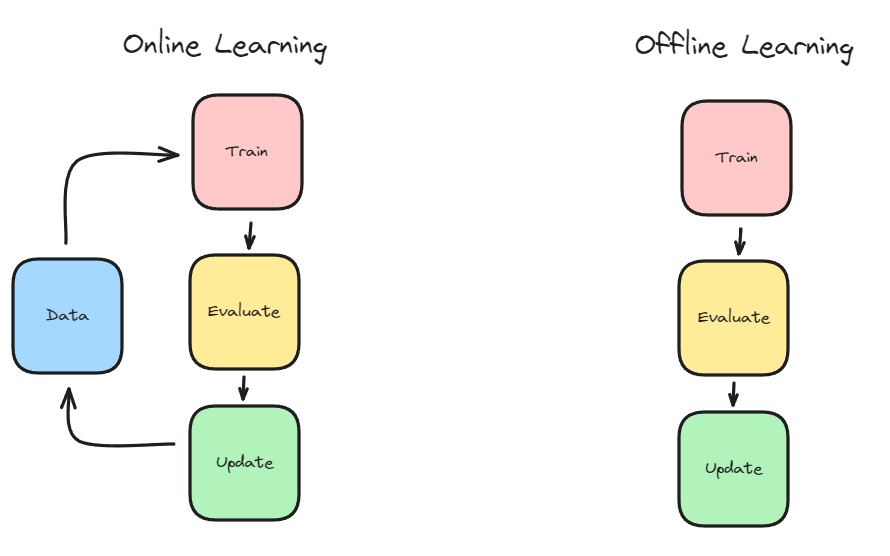
\includegraphics[width=1\textwidth]{images/online_vs_offline_learning.png}
    \caption{Online Learning ve Offline Learning..}
    \label{fig:enter-label}
\end{figure}

\subsection{Offline Learning}
Model bir veri seti üzerinde eğitilir ve eğitildikten sonra sabit kalır. Yeni veri geldiğinde, model güncellenmez ve bu nedenle yeni bilgileri öğrenme yeteneği sınırlıdır.

\subsection{Continual Learning (Sürekli Öğrenme)}
Bir modelin zaman içinde gelen yeni veri ile sürekli olarak güncellenerek öğrenmeye devam ettiği bir yöntemdir. Model başlangıçta öğrendiği bilgileri sürekli olarak genişletir ve günceller. Model, yeni veriyi öğrenirken önceki bilgileri unutma eğilimindedir. Bu bilgi çakışmasına (catastrophic forgetting) neden olabilir. Bunu önlemek için ağ yeniden kullanılır (network reuse). Önceki eğitilmiş ağ, yeni veri üzerinde eğitim yapmak için kullanılır.

\subsection{Incremental Learning (Artımlı Öğrenme)}
Bir modelin önceki eğitimin genişletmek veya yeni sınıflar ekleyerek güncellenmesine dayanır.

\subsection{Modeller}
Parametreler: fit\_partial, warm\_start, init\_model \\
'fit\_partial' parametresi ile eğitilenler:
\begin{itemize}
    \item MultinomialNB
    \item BernoulliNB
    \item Perceptron
    \item SGDClassifier
    \item PassiveAggressiveClassifier
    \item SGDRegressor
    \item PassiveAggressiveRegressor
    \item MiniBatchKMeans
\end{itemize}

'init\_model' parametresi ile eğitilenler:
\begin{itemize}
    \item LGBMClassifier
    \item XGBClassifier
    \item CatBoostClassifier
    \item LGBMRegressor
    \item XGBRegressor
    \item CatBoostRegressor
\end{itemize}

\newpage